\subsection{First Current Mirror Circuit}
% Current mirror 1
\FloatBarrier

\begin{figure}[h!]
	\centering
	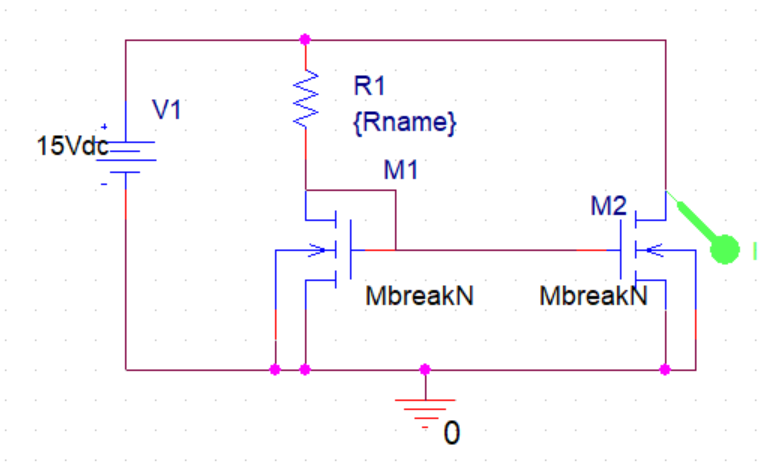
\includegraphics[scale=0.75]{./images/circuit4.PNG}
	\caption{First Current Mirror Circuit}
	\label{fig:circuit4}
\end{figure}

\FloatBarrier

% How the current mirror works
Assume transistors $M_1$ and $M_2$ in figure (\ref{fig:circuit4}) are identical. Because $M_1$ is a diode-connected MOSFET, if $V_{DS} = V_{GS} > V_T$, then $M_1$ operates in saturation. If $R_1$ is sufficiently small, then $V_R$ can be small enough that $V_{DS} > V_T$. $M_1$'s drain current shall be called $i_{ref}$, and $M_2$'s $i_{out}$. \\

Because the gates of $M_1$ and $M_2$ are connected and both of their sources are grounded, $V_{GS}$ is the same for each. Since $M_1$ and $M_2$ are identical transistors, their $V_{T}$ values are identical as well. So, if current can flow through $M_1$'s drain, then $M_2$ must also be active because $V_{GS} >= V_{T}$ in both cases. $M_2$'s $V_{DS}$ certainly exceeds $M_1$'s $V_{DS}$ since $M_2$'s drain is directly connected to the supply voltage rather than an intermediary resistor. Since $M_1$ is in saturation, $V_{DS} >= V_{GS} - V_{T}$ is the condition for saturation, and $M_2$'s $V_{DS}$ exceeds $M_1$'s $V_{DS}$, then $M_2$ must also be in saturation. \\

Since both transistors are in saturation, have the same $V_{GS}$ value, and have identical structures, the following must be true:

\begin{equation}
	\label{eq:current_mirror_eqn}
	\frac{ i_{ref} }{ i_{out} } = \frac{ \frac{k_n}{2} ( V_{GS} - V_{T} )^2 }{ \frac{k_n}{2} ( V_{GS} - V_{T} )^2 } = 1 \rightarrow i_{ref} = i_{out}
\end{equation}

This circuit is called a "current mirror" because of the property demonstrated in equation (\ref{eq:current_mirror_eqn}). Given any input current $i_{ref}$, the output current $i_{out}$ must be the same. Changing the dimensions of the transistors relative to one another can alter the output current by a constant factor \cite{current_src_dim}. \\

% Why the I vs. R relationship

\FloatBarrier

\begin{figure}[h!]
	\centering
	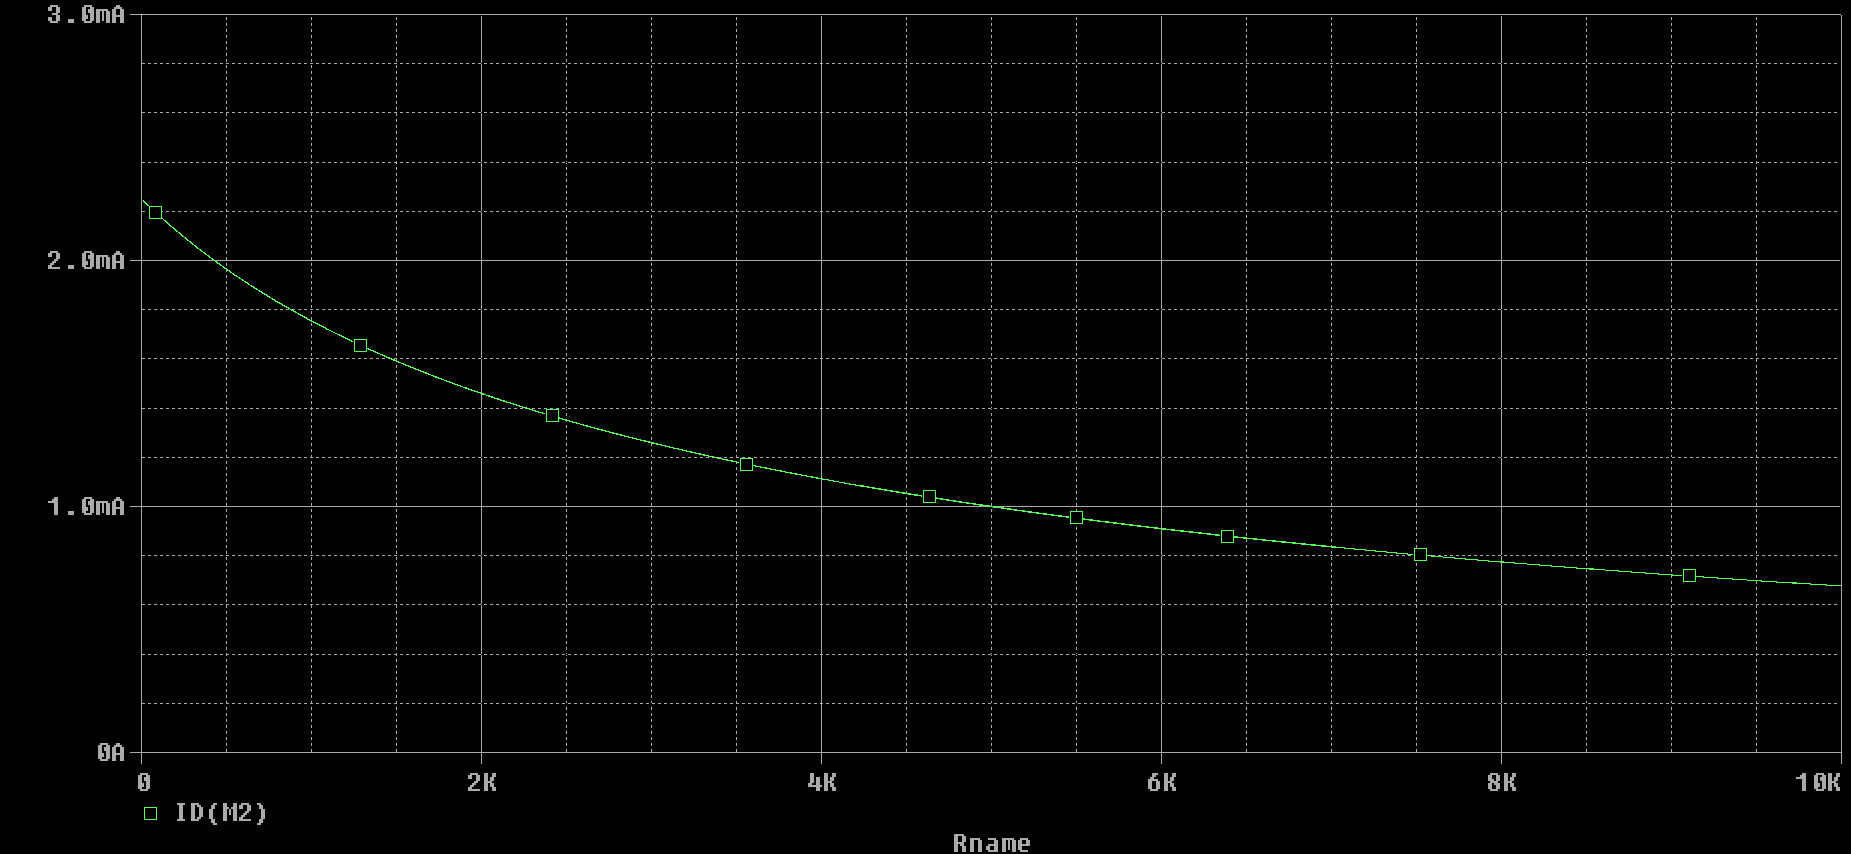
\includegraphics[scale=0.5]{./images/circuit4_r_sweep.PNG}
	\caption{$i_{out}$ versus $R_1$ for Current Mirror in Figure (\ref{fig:circuit4})}
	\label{fig:circuit4_r_sweep}
\end{figure}

\FloatBarrier

In the extreme case of an open circuit in the place of $R_1$, the open circuit absorbs the supply voltage, leaving none for $M_1$. So, $V_{DS} = V_{GS} = 0$. For these NMOS transistors, $V_{T} > 0$ (confirm detail with a reference). Therefore, $V_{GS} < V_{T}$. So, $M_1$ is operating in the cutoff region, and no current flows. \\

On the other hand, if $R_1$ is a short and $V_{T} < V_{DD}$ (as it should be), where $V_{DD}$ is the supply voltage, then $V_{GS} = V_{DD} > V_{T}$. Thus, $M_1$ is enabled. Because $M_1$ is diode-connected, it operates in the saturation region. Thus, as $R_1$ is increased, it absorbs more and more of the supply voltage $V_{DD}$ until $M_1$ operates in cutoff mode. Thus, the $i_{ref}$ versus $R_1$ curve should be downward sloping.\\

\subsection{Second Current Mirror Circuit}
% Current mirror 2

\FloatBarrier

\begin{figure}[h!]
	\centering
	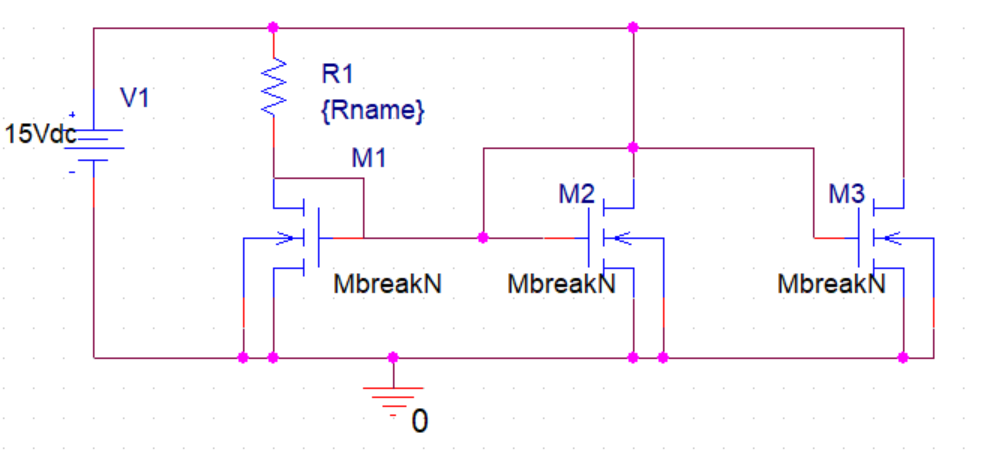
\includegraphics[scale=0.75]{./images/circuit5.PNG}
	\caption{Second Current Mirror Circuit}
	\label{fig:circuit5}
\end{figure}

\FloatBarrier

Consider the transistor $M_1$. $V_G = 15$\si{\volt} and $V_S = 0$\si{\volt}. Therefore, $V_{GS,M1}$ is likely much larger than $V_{T,M1}$. As a result, the transistor is active. Because $M_1$ is active and is diode-connected, $M_1$ must be in saturation. By the same arguments, $M_2$ and $M_3$ are also operating in saturation.\\

Both terminals of $R_1$ have the same potential due to the short path leading from the supply voltage lane to $M_1$'s drain terminal. So, by Ohm's Law, no current flows through the resistor $R_1$. So, the circuit's operation is technically identical regardless of the value of $R_1$ in place. $R_1$ always acts as a short. Therefore, the plots of drain current versus $R_1$ should be constant for any of the transistors.\\

Because $M_1$ is in saturation, $i_{D,M1} = \frac{ k_n }{ 2 } ( V_{GS,M1} - V_{T,M1} )^2$. Because $V_{GS,M1}$ is so large in comparison to $V_{T,M1}$ due to $M_1$'s terminals being directly connected to the supply voltage lane, $i_{D,M1}$ should not be $0$\si{\milli\ampere}. $M_1$ draws this current from the supply voltage through the short path to its gate to its drain, bypassing the resistor $R_1$.\\

All of the transistors are identical in the sense that the voltages applied at the gate, source, and drain are the same. Thus, the drain current through each transistor is the same. So, the drain current through $M_1$ should be significant and constant when varied with $R_1$. The sum of the drain currents through $M_2$ and $M_3$ should also be double the drain current through $M_1$ and constant when varied with $R_1$. This is because the drain current curves are the same for $M_2$ and $M_3$ as they are for $M_1$. Therefore, adding them together simply doubles the constant drain current for all $R_1$ values.\\

\FloatBarrier

\begin{figure}[h!]
	\centering
	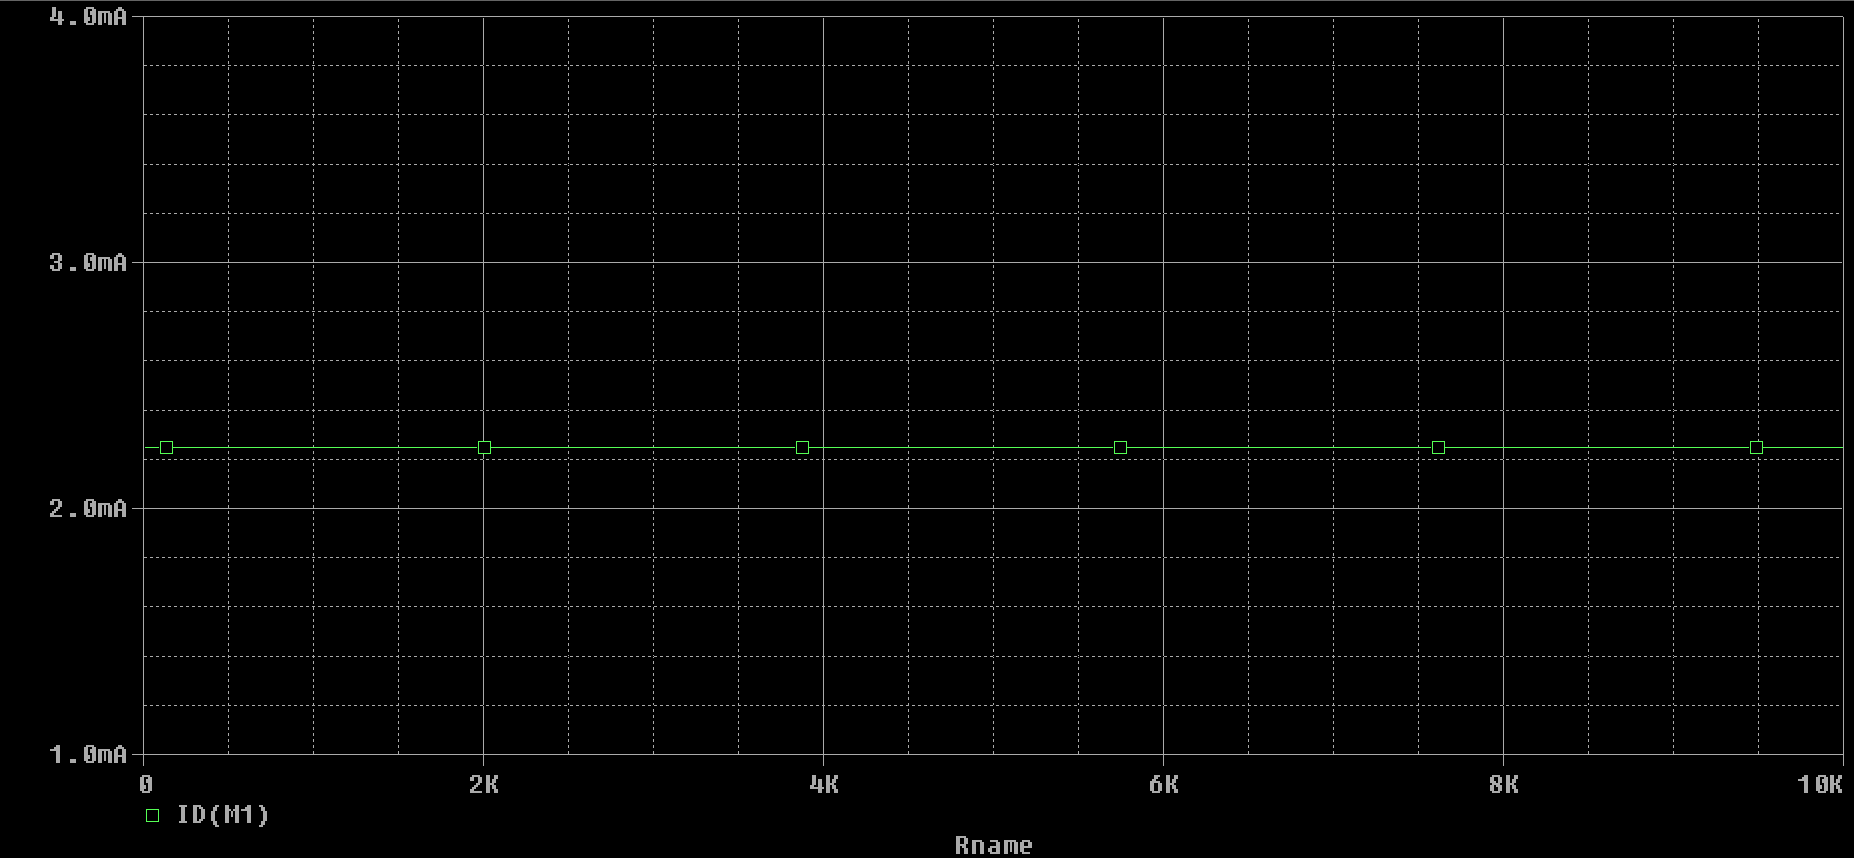
\includegraphics[scale=0.5]{./images/circuit5_id1_vs_r.PNG}
	\caption{$i_{D,M1}$ versus $R_1$}
	\label{fig:circuit5_id1_vs_r}
\end{figure}

\FloatBarrier

\FloatBarrier

\begin{figure}[h!]
	\centering
	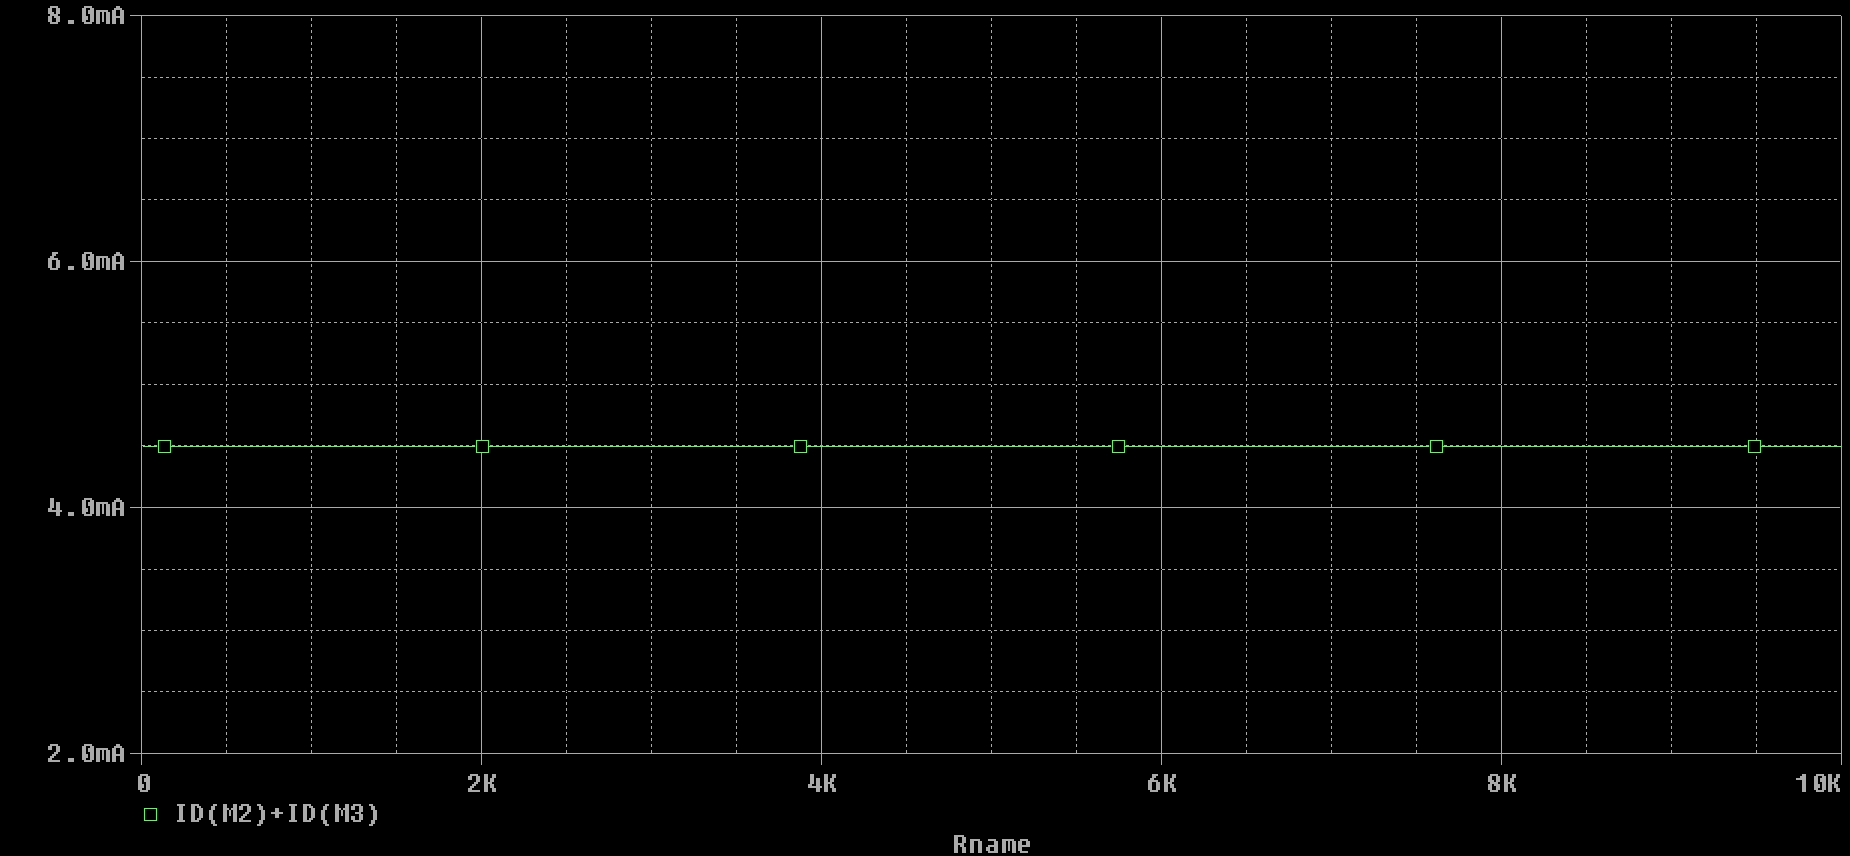
\includegraphics[scale=0.5]{./images/circuit5_id2_plus_id3_vs_r.PNG}
	\caption{$i_{D,M2} + i_{D,M3}$ versus $R_1$}
	\label{fig:circuit5_id2_plus_id3_vs_r}
\end{figure}

\FloatBarrier

The results of the simulation are consistent with this analysis. In figure (\ref{fig:circuit5_id1_vs_r}), the current value is essentially $2.25$\si{\milli\ampere}, a significant current value through the drain of $M_1$. In figure (\ref{fig:circuit5_id2_plus_id3_vs_r}), the current value is nearly twice that, approximately $4.5$\si{\milli\ampere}. In both cases, the drain currents are not functions of the resistance $R_1$.
